\documentclass{standalone}
\usepackage{tikz}
\usepackage{textcomp}

\begin{document}

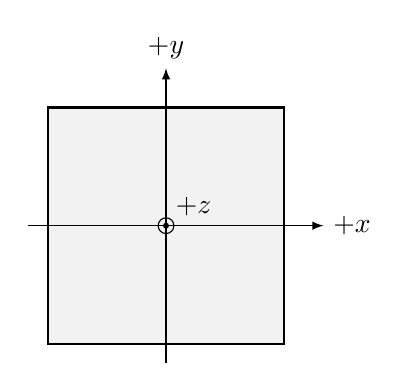
\begin{tikzpicture}

\draw [thick, fill=gray, fill opacity=0.1] (0,0) -- (3,0) -- (3,3) -- (0,3) -- cycle;
\draw[-latex] (-0.25,1.5) -- (3.5,1.5);
\node [right] at (3.5, 1.5) {$+x$};
\draw[-latex] (1.5,-0.25) -- (1.5,3.5);
\node [above] at (1.5, 3.5) {$+y$};
\draw[fill=black] (1.5,1.5) circle [radius=0.03];
\draw (1.5,1.5) circle [radius=0.1];
\node [above right] at (1.5, 1.5) {$+z$};

\end{tikzpicture}
\end{document}
